\documentclass{rapportECL}
\usepackage{lipsum}
\usepackage{overpic}
\usepackage{xcolor}
\usepackage{graphicx}
\usepackage{tcolorbox}
\usepackage[utf8]{inputenc}
\usepackage[T1]{fontenc}
\usepackage[french]{babel}
\usepackage{amsmath}
\usepackage{amsfonts}
\usepackage{amssymb}
\usepackage{geometry}
\usepackage{listings}
\usepackage{xcolor}
\usepackage{hyperref}
\usepackage{siunitx}      % Pour les unités avec \SI
\usepackage{float}        % Pour le placement [H] des figures
\title{Rapport ECL - Template} %Titre du fichier

\begin{document}

%----------- Informations du rapport ---------

\titre{Couplage multiphysique thermo-mécanique : étude et simulation numérique sous ANSYS} %Titre du fichier .pdf
% \UE{ DIMENSIONNEMENT DES STRUCTURES} %Nom de la UE
\enseignant{Saadlaoui \textsc{Yassine}} %Nom de l'enseignant


\eleves{Kevin \textsc{TONGUE}\\ BIAOU \textsc{Adebayo Landry}\\ Gaston \textsc{KAMDEM TCHOMTHOUA} }
\UE{ENISE-5GM}


% \eleves{Kevin \textsc{TONGUE} }
\UEU{ENISE-4GM}

%----------- Initialisation -------------------
        
\fairemarges %Afficher les marges
\fairepagedegarde %Créer la page de garde
\tabledematieres %Créer la table de matières


\section{Introduction}

Ce rapport présente les étapes et les résultats d’une simulation numérique réalisée avec ANSYS Workbench, dans le cadre de l’étude du couplage multiphysique appliqué aux procédés industriels. L’objectif principal est de modéliser l’effet d’un flux de chaleur mobile sur une plaque rectangulaire à l’aide d’une analyse thermique transitoire, en vue de préparer un futur couplage thermo-mécanique. La méthodologie adoptée suit le flux de travail standard d’ANSYS, depuis la conception géométrique jusqu’à l’exploitation des résultats obtenus.

\subsection{Contexte et objectifs du TP}

Dans le cadre du cours sur le couplage multiphysique pour les procédés, ce travail pratique a pour objectif de simuler un procédé thermique impliquant une source de chaleur mobile. Ce type de chargement est représentatif de nombreux procédés industriels, tels que le soudage, la découpe laser ou le traitement thermique localisé.

\textbf{Objectifs :}
\begin{itemize}
    \item \textbf{Objectif principal :} Étudier la distribution transitoire de la température dans une plaque rectangulaire soumise à un flux de chaleur mobile, à l’aide d’une analyse \texttt{Transient Thermal}.
    \item \textbf{Objectif secondaire (couplage) :} Préparer le modèle pour une analyse thermo-mécanique ultérieure, où les champs de température obtenus serviront de chargement pour l’évaluation des contraintes résiduelles et des déformations.
    \item \textbf{Prise en main :} Se familiariser avec l’environnement ANSYS Workbench, depuis la création de la géométrie jusqu’à l’exploitation et l’interprétation des résultats.
\end{itemize}

\section{Présentation du logiciel ANSYS Workbench}

ANSYS Workbench est une plateforme de simulation numérique intégrée par éléments finis, largement utilisée en ingénierie. Elle se distingue par sa capacité à gérer des projets complexes et à intégrer plusieurs disciplines physiques au sein d’un même environnement, facilitant ainsi les études de \textbf{couplage multiphysique}.

\subsection{Architecture et interface}

Workbench propose une interface graphique intuitive :  
\begin{itemize}
    \item \textbf{Toolbox (Boîte à outils)} : Contient les différents types d’analyses et systèmes disponibles (structural, thermique, CFD, électromagnétique, etc.).  
    \item \textbf{Project Schematic (Schéma projet)} : Espace central où les analyses sont représentées par des blocs connectables, permettant le partage de données et la création de workflows multiphysiques.
\end{itemize}

\subsection{Systèmes d'analyse}

ANSYS Workbench regroupe les analyses par grandes familles :  
\begin{itemize}
    \item \textbf{Structures et thermique} : Analyses statiques, dynamiques et thermiques (stationnaire et transitoire).  
    \item \textbf{Fluide (CFD)} : Simulation des écoulements et transferts thermiques avec \textbf{Fluent} ou \textbf{CFX}.  
    \item \textbf{Électromagnétisme} : Simulation des champs électriques et magnétiques avec \textbf{Maxwell}.  
\end{itemize}

\subsection{Couplage multiphysique}

Workbench permet d’étudier l’interaction entre plusieurs phénomènes physiques :  
\begin{itemize}
    \item \textbf{Couplage séquentiel (1-way)} : Les résultats d’une analyse (ex. température) servent de chargement pour une autre (ex. mécanique).  
    \item \textbf{Couplage bidirectionnel (2-way)} : Les interactions se font dans les deux sens, par exemple en interaction fluide-structure via \textbf{System Coupling}.
\end{itemize}

\subsection{Environnement ANSYS Mechanical}

Dans ANSYS Mechanical, l’utilisateur prépare et résout les simulations :  
\begin{itemize}
    \item Maillage des géométries pour optimiser précision et temps de calcul.  
    \item Application des conditions aux limites et chargements spécifiques (ex. source de chaleur mobile).  
    \item Résolution et analyse des résultats (déformations, contraintes, distributions de température, etc.).
\end{itemize}

ANSYS Workbench constitue ainsi un outil complet et flexible pour la simulation de phénomènes complexes et le couplage multiphysique.

\section{Méthodologie}

La méthodologie adoptée suit rigoureusement le flux de travail proposé par le schéma projet dans ANSYS Workbench, en débutant par une analyse \textbf{thermique transitoire}.

\subsection{Sélection du système d’analyse}

Pour modéliser un flux de chaleur mobile, une analyse de type \textbf{\texttt{Transient Thermal}} a été sélectionnée. Ce système est le plus approprié car il permet de calculer l’évolution de la température en fonction du temps, ce qui est essentiel pour suivre le déplacement de la source chaude sur la pièce.

\begin{figure}[H]
    \centering
    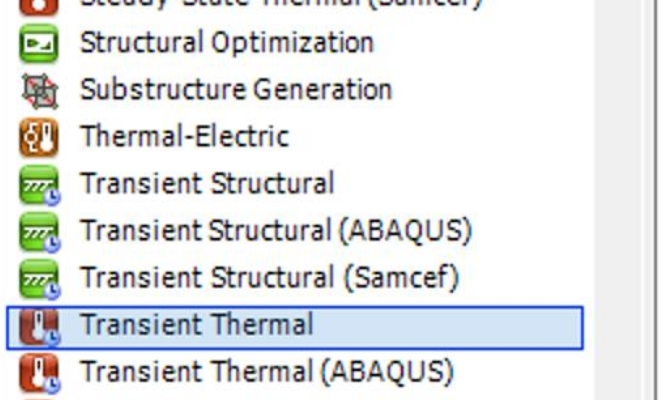
\includegraphics[width=0.5\linewidth]{i_ansys2.png}
    \caption{Sélection d'un système d'analyse dans la toolbox.}
    \label{fig:toolbox}
\end{figure}

\begin{figure}[H]
    \centering
    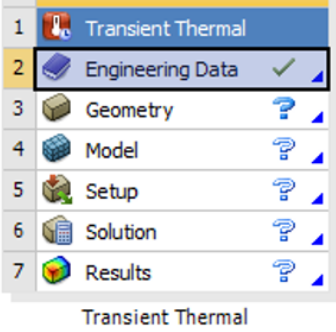
\includegraphics[width=0.5\linewidth]{i_ansys3.png}
    \caption{Analyse de type Transient Thermal dans le Project Schematic.}
    \label{fig:transient}
\end{figure}

\subsection{Définition des données matériau (Engineering Data)}

Pour garantir la précision des résultats, un nouveau matériau a été créé. En s’appuyant sur des données issues de la littérature, les propriétés suivantes, essentielles pour une analyse thermique, ont été définies :

\begin{itemize}
    \item \textbf{Densité} : valeur scalaire constante.
    \item \textbf{Conductivité thermique isotrope} : éventuellement définie comme fonction de la température.
    \item \textbf{Chaleur spécifique à pression constante} : éventuellement définie comme fonction de la température.
\end{itemize}

L’importation de données tabulées a permis de reproduire fidèlement le comportement physique réel du matériau.

\subsection{Création de la géométrie (SpaceClaim)}

La géométrie de la pièce a été réalisée sous \textbf{SpaceClaim}, l’outil de modélisation intégré à ANSYS.
\begin{itemize}
    \item \textbf{Forme :} Une plaque rectangulaire a été esquissée en 2D à l’aide de l’outil \texttt{Rectangle}.
    \item \textbf{Dimensionnement} 
    \item \textbf{Extrusion :} L’outil \texttt{Pull} a été utilisé pour extruder la surface et donner une épaisseur à la plaque, créant ainsi un volume 3D.
\end{itemize}

\begin{figure}[H]
    \centering
    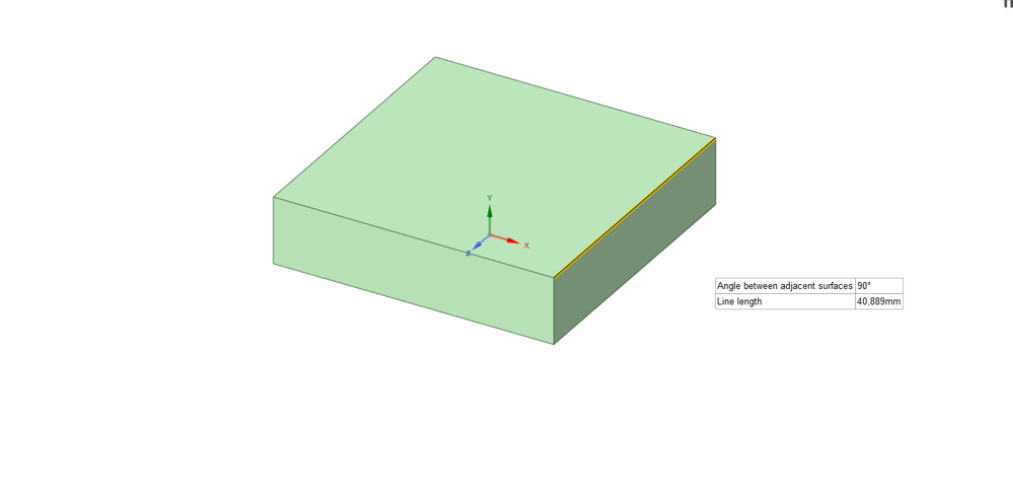
\includegraphics[width=0.75\linewidth]{i_ansys4.png}
    \caption{Géométrie de la plaque réalisée sous SpaceClaim.}
    \label{fig:geom}
\end{figure}

\subsection{Mise en données du modèle (Model)}

L’étape suivante, réalisée dans \textbf{ANSYS Mechanical}, consiste à préparer le modèle pour le calcul.

\begin{itemize}
    \item \textbf{Affectation du matériau :} Le matériau choisi est l’\textbf{acier structural} (matériau par défaut d’ANSYS), que nous avons assigné au volume de la pièce.
    \item \textbf{Maillage (Mesh) :} Un maillage de type \texttt{Body Sizing} a été appliqué à la géométrie. Nous avons considéré un maillage \textbf{hexaédrique} afin d’uniformiser la distribution des éléments et de faciliter la convergence des résultats. La taille des éléments a été choisie de façon contrôlée pour obtenir un compromis optimal entre précision (notamment dans la zone du cordon de chaleur) et temps de calcul.
\end{itemize}

\begin{figure}[H]
    \centering
    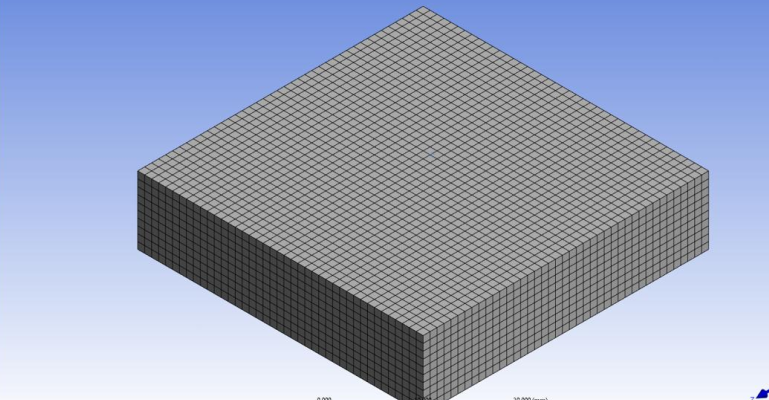
\includegraphics[width=0.75\linewidth]{i_ansys5.png}
    \caption{Maillage de la plaque.}
    \label{fig:mesh}
\end{figure}

\subsection{Configuration du calcul (Setup)}

Après insertion de l’extension \textbf{Moving Heat Source} via l’outil ACT, les différentes étapes de configuration ont été réalisées comme suit :

\begin{itemize}
    \item \textbf{Application de la convection thermique :} 
    Une condition de convection a été appliquée sur les surfaces exposées à l’air ambiant afin de modéliser les échanges thermiques avec l’environnement. 
    Un coefficient de convection thermique de \SI{0.048}{W/m^2.K} a été considéré.

    \item \textbf{Définition du flux de chaleur mobile :} 
    Le chargement thermique a été introduit à l’aide de l’option \texttt{Moving Heat Source}. 
    Le flux de chaleur a été appliqué au matériau en définissant :
    \begin{itemize}
        \item la \textbf{géométrie cible} (scope),
        \item le \textbf{chemin de déplacement} correspondant à la longueur de la pièce,
        \item un \textbf{point de départ} définissant l’origine du mouvement,
        \item la \textbf{direction de propagation} suivant la longueur de la pièce,
        \item la \textbf{vitesse de déplacement} du flux thermique.
    \end{itemize}

    \item \textbf{Paramètres temporels :}
    Le temps de début et le temps de fin d’application du flux ont été définis en cohérence avec la vitesse de déplacement et la longueur du trajet, afin d’assurer une évolution réaliste de la source thermique. 
    Le nombre de sous-pas (substeps) a également été ajusté pour garantir une bonne résolution temporelle du phénomène, notamment durant la phase de chauffage et de refroidissement.

    \item \textbf{Lancement du calcul :}
    Après validation de l’ensemble des paramètres (conditions aux limites, chargement et paramètres temporels), le solveur a été exécuté pour obtenir les champs de température transitoires.
\end{itemize}

\begin{figure}[H]
    \centering
    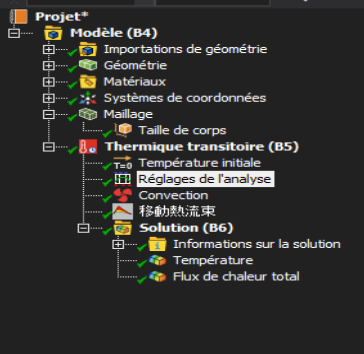
\includegraphics[width=0.5\linewidth]{i_ansys6.png}
    \caption{Arborescence du modèle d’analyse thermique transitoire dans ANSYS Mechanical.}
    \label{fig:tree}
\end{figure}

\subsection{Couplage thermo-mécanique}

Afin d’évaluer les effets mécaniques induits par le cycle thermique, un couplage thermo-mécanique a été mis en place. L’analyse mécanique est basée sur les résultats de l’analyse thermique transitoire précédemment réalisée.

\subsubsection{Mise en place du couplage dans Workbench}

Dans ANSYS Workbench, un système \textbf{Static Structural} a été ajouté et relié au système \textbf{Transient Thermal}. Le couplage est réalisé en connectant la cellule \texttt{Solution} de l’analyse thermique à la cellule \texttt{Setup} de l’analyse mécanique. Cette liaison permet de transférer automatiquement le champ de température calculé comme chargement thermique dans l’étude mécanique. Ainsi, la température devient une charge appliquée au modèle structurel.

\begin{figure}[H]
    \centering
    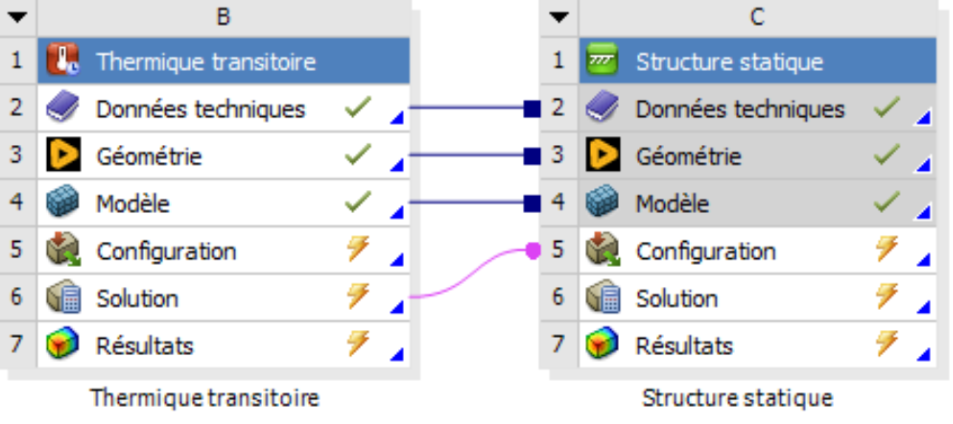
\includegraphics[width=0.5\linewidth]{i_asys7.png}
    \caption{Couplage dans ANSYS Workbench entre l’analyse thermique transitoire et l’analyse structurelle statique.}
    \label{fig:couplage}
\end{figure}

\subsubsection{Conditions aux limites mécaniques}

Après importation du champ thermique (\texttt{Imported Temperature}), les conditions mécaniques suivantes ont été définies :

\begin{itemize}
    \item \textbf{Encastrement (Fixed Support)} sur une face de la plaque afin de simuler un maintien rigide.
    \item Les autres faces restent libres afin de permettre la dilatation thermique du matériau.
\end{itemize}

\begin{figure}[H]
    \centering
    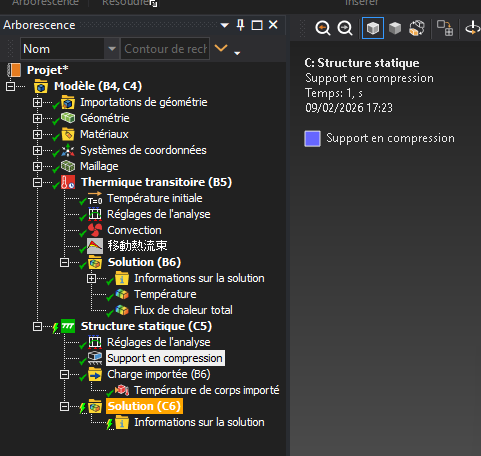
\includegraphics[width=0.75\linewidth]{i_.png}
    \caption{Arborescence du couplage entre les systèmes Thermique transitoire et Structure statique}
    \label{fig:placeholder}
\end{figure}


\section{Résultats et discussion}

Les calculs ont été menés sur une plaque parallélépipédique de dimensions 50 x 20 x 10 mm en aluminium, soumise à un flux de chaleur mobile d’environ \SI{600}{W/mm^2} se déplaçant sur la face supérieure, avec une convection externe d’environ \SI{50}{W/m^2.K}. Les résultats sont présentés ci-dessous.

\subsection{Analyse thermique}

La figure \ref{fig:thermique} montre la distribution de température à un instant donné. On observe clairement le déplacement de la zone chaude, avec un gradient thermique important en tête de la source et un refroidissement progressif derrière celle-ci. L’animation temporelle (non reproduite ici) confirme la propagation réaliste de la source.

\begin{figure}[H]
    \centering
    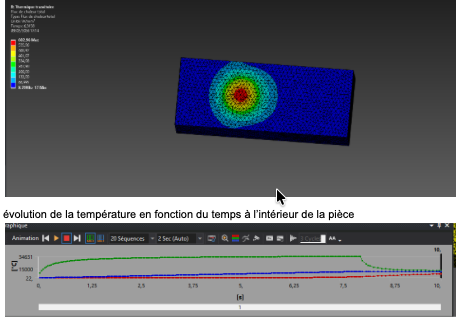
\includegraphics[width=1\linewidth]{Images saadlaoui/résultat thermique.png}
    \caption{Champ de température transitoire lors du passage de la source de chaleur mobile.}
    \label{fig:thermique}
\end{figure}

\subsection{Analyse mécanique (couplage)}

Les champs de température ont ensuite été utilisés comme chargement dans l’analyse statique structurelle. Les figures suivantes présentent les principaux résultats mécaniques.

\begin{figure}[H]
    \centering
    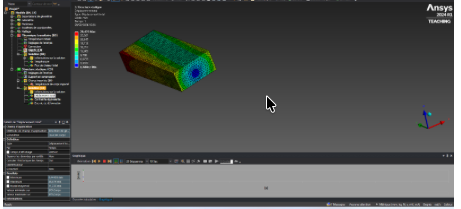
\includegraphics[width=1\linewidth]{Images saadlaoui/couplage déplacement total.png}
    \caption{Déplacement total de la plaque sous l'effet de la dilatation thermique.}
    \label{fig:deplacement}
\end{figure}

\begin{figure}[H]
    \centering
    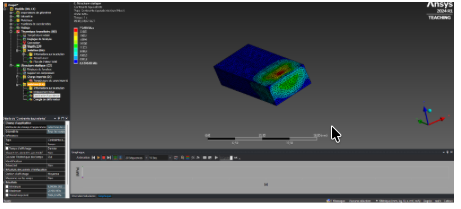
\includegraphics[width=1\linewidth]{Images saadlaoui/couplage contrainte équivalente de Von Mises.png}
    \caption{Contrainte équivalente de Von Mises induite par le cycle thermique.}
    \label{fig:contrainte}
\end{figure}

\begin{figure}[H]
    \centering
    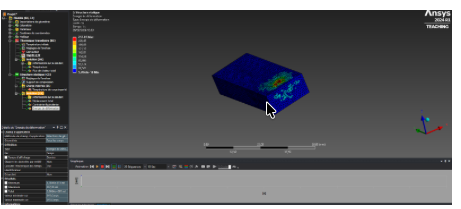
\includegraphics[width=1\linewidth]{Images saadlaoui/couplage energie de deformation.png}
    \caption{Énergie de déformation totale dans la plaque.}
    \label{fig:energie}
\end{figure}

\subsection{Interprétation}

Les résultats montrent une concentration de contraintes et de déformations dans la zone affectée thermiquement. La contrainte de Von Mises atteint des valeurs significatives, ce qui pourrait conduire à l’apparition de contraintes résiduelles après refroidissement. L’énergie de déformation reflète l’intensité de la sollicitation mécanique due au gradient thermique.

\subsection{Difficultés rencontrées}

Lors de la mise en œuvre de la simulation, plusieurs difficultés ont été rencontrées :
\begin{itemize}
    \item Une première approche consistant à modéliser le flux de chaleur mobile à l’aide de scripts personnalisés (code utilisateur ou commandes APDL) a été tentée. Malgré de nombreux ajustements et une prise de temps conséquente, les résultats obtenus n’étaient pas satisfaisants et ne correspondaient pas aux attendus physiques.
    \item Face à cet échec, nous nous sommes tournés vers l’extension dédiée \texttt{Moving Heat Source} disponible sur la plateforme ANSYS. Toutefois, l’interface de cette extension était en chinois/japonais, ce qui a rendu la saisie des paramètres délicate et a nécessité une vigilance accrue pour éviter toute erreur de configuration. Finalement, cette extension a permis d’obtenir les résultats escomptés.
\end{itemize}


\section{Conclusion}

Ce travail a permis de modéliser un procédé thermique à source de chaleur mobile sous ANSYS Workbench à travers une analyse \textbf{Transient Thermal}, puis de mettre en place un couplage thermo-mécanique séquentiel afin d’évaluer les contraintes et déformations induites. L’étude a nécessité la maîtrise complète de la chaîne de simulation : définition des propriétés matériau, maillage contrôlé, paramétrage temporel et implémentation d’un flux thermique mobile via une extension ACT. Les résultats obtenus mettent en évidence l’influence du cycle thermique sur le comportement mécanique de la pièce et soulignent l’importance de la qualité du maillage ainsi que de la précision des données matériau pour garantir la fiabilité des simulations. Cette démarche constitue une base solide pour des analyses multiphysiques plus avancées et l’optimisation des procédés thermiques.

\newpage

\section{Synthèse des travaux scientifiques présentés par les autres groupes et corrélations avec notre travail}

\subsection{Résumé des documents scientifiques}

Deux documents scientifiques ont été étudiés pour enrichir notre compréhension des modélisations thermiques avancées.

\subsubsection{Article principal : "A Temperature-Dependent Heat Source for Simulating Deep Penetration in Selective Laser Melting Process"}

Cet article, publié dans \textit{Applied Sciences} en 2021, propose une nouvelle méthode de simulation numérique pour le procédé de fusion laser sélective (SLM). Les auteurs (Y. Jia et al.) constatent que les modèles thermiques classiques par éléments finis, bien qu’efficaces pour prédire les distorsions et contraintes résiduelles à l’échelle macroscopique, négligent les effets de la convection dans le bain de fusion et les phénomènes de keyhole. Il en résulte une sous-estimation de la profondeur du bain et une surestimation de sa largeur.

Pour remédier à cette limitation, ils développent une \textbf{source de chaleur dépendante de la température} dont les paramètres s’ajustent automatiquement au cours de la simulation. Concrètement, la profondeur de pénétration \(\eta_t\) et la position de la puissance maximale \(z_0\) sont recalibrées à chaque pas de temps en fonction de la température moyenne d’un volume de contrôle situé sous le faisceau. Ce mécanisme permet de compenser les effets thermiques non modélisés (écoulements, réflexions multiples) sans recourir à des simulations multiphysiques lourdes.

Les résultats obtenus pour deux matériaux (AlSi10Mg et Inconel 718) montrent une excellente concordance avec les mesures expérimentales : l’erreur relative est inférieure à 5\% pour la profondeur du bain. De plus, la méthode s’avère peu sensible au choix du pas de temps et ne nécessite qu’une calibration unique par matériau (pour \(z_0\)). Elle constitue donc une alternative efficace et facile à implémenter par rapport aux techniques classiques comme la conductivité thermique anisotrope.

\subsubsection{Corrigendum : "Corrigendum to Case Stud. Therm. Eng. 35 2022 102078"}

Ce court document corrige deux erreurs présentes dans un article antérieur. La première concerne l’équation (2) décrivant la source de chaleur, qui est désormais correctement formulée sous forme d’une exponentielle gaussienne 3D. La seconde clarifie la décomposition de la déformation globale en parties élastique, (visco)plastique et thermique, ainsi que la relation contrainte-déformation via le tenseur de compliance. Ces corrections soulignent l’importance de la rigueur mathématique et dimensionnelle dans les modèles thermomécaniques.

\subsection{Corrélation avec notre travail}

Notre étude sous ANSYS Workbench partage des objectifs communs avec ces travaux de recherche. Dans les deux cas, il s’agit de modéliser une source de chaleur mobile pour obtenir un champ de température réaliste, condition essentielle à une analyse mécanique fiable.

- **Représentation de la source** : Dans l’article, la source adaptative améliore la précision en tenant compte indirectement des phénomènes complexes. Dans notre simulation, l’utilisation de l’extension \texttt{Moving Heat Source} a permis de définir un flux mobile avec un chemin, une vitesse et une distribution spatiale, même si l’interface était en chinois. Cette étape illustre la difficulté pratique de paramétrer correctement une source thermique.
- **Couplage thermo-mécanique** : Les deux approches aboutissent à un transfert des températures vers un calcul mécanique (contraintes, déformations). L’article valide l’importance de la précision thermique pour la prédiction des grandeurs mécaniques, ce que nous avons également constaté dans nos résultats (concentration de contraintes dans la zone affectée).
- **Perspectives** : La méthode proposée dans l’article pourrait être implémentée dans des travaux futurs sous ANSYS, par exemple via des scripts APDL, pour simuler des phénomènes de pénétration profonde (keyhole) sans recourir à des modèles multiphysiques coûteux. Cela ouvrirait la voie à des simulations plus réalistes de procédés comme le soudage laser ou la fusion laser sur lit de poudre.

En conclusion, l’étude de ces documents scientifiques a renforcé notre compréhension des enjeux liés à la modélisation thermique et a confirmé la pertinence de notre démarche de couplage séquentiel sous ANSYS Workbench.

\section{Sources utilisées}

\begin{itemize}
    \item Tutoriel ANSYS Workbench – source de chaleur mobile : \url{https://www.youtube.com/watch?v=LqWSRqnFyn8}
    \item Tutoriel complémentaire – couplage thermomécanique : \url{https://www.youtube.com/watch?v=2PIu2-JOluk}
\end{itemize}

\end{document}